\ifdefined\included
\else
\documentclass[french, a4paper, 11pt, twoside, pdftex]{StyleThese}
\usepackage{iflang}
\usepackage{bibentry}



%\usepackage[sectionbib]{chapterbib}          % Cross-reference package (Natural BiB)
%\usepackage{natbib}                  % Put References at the end of each chapter
%\usepackage{bibunits}
% Do not put 'sectionbib' option here.
% Sectionbib option in 'natbib' will do.


\usepackage{fancyhdr}                    % Fancy Header and Footer

\usepackage[utf8]{inputenc}
\usepackage[T1]{fontenc}
\usepackage[french]{babel} %
\usepackage{lmodern} \normalfont %to load T1lmr.fd 
\DeclareFontShape{T1}{cmr}{b}{sc} { <-> ssub * cmr/bx/sc }{}
%\hyphenation{gar}

\usepackage{amsmath,amssymb}             % AMS Math
\usepackage{nicefrac}
\usepackage{siunitx}					%% Unites Math SI

\usepackage{blindtext}

\usepackage{datetime}

\usepackage{lipsum} 

\usepackage[inline]{enumitem}

\usepackage{hhline}
%\usepackage[left=1.5in,right=1.3in,top=1.1in,bottom=1.1in]{geometry}
\usepackage[left=1.5in,right=1.3in,top=1.1in,bottom=1.1in,includefoot,includehead,headheight=13.6pt]{geometry}

%%\renewcommand{\baselinestretch}{1.05}

%%%%%%%% Multi-figures avec sub-captions
\usepackage{caption}
\usepackage{subcaption}

% Table of contents for each chapter

\usepackage[nottoc, notlof, notlot]{tocbibind}
\usepackage[nohints]{minitoc}
\setcounter{minitocdepth}{2}
\mtcindent=15pt
% Use \minitoc where to put a table of contents

\usepackage{aecompl}

%% Package cosmetic meilleur layout du texte en jouant sur le spacing par caractères
\usepackage[activate={true,nocompatibility},final,tracking=true,kerning=true,factor=1100,stretch=10,shrink=10]{microtype}
\usepackage[absolute,overlay]{textpos} 
\setlength{\TPHorizModule}{\paperwidth}\setlength{\TPVertModule}{\paperheight}
\sloppy

%%%%%%%%%%% JOLIS TABLEAUX
\usepackage{tabularx}		%\usepackage{tabular}
\usepackage{longtable}
\usepackage{multirow}
\newcommand{\mc}{\multicolumn} 
\newcommand{\mr}[2]{\multirow{#1}{*}{#2}} 	\newcommand{\mrQ}{\multirow{-4}{*}}
\usepackage{booktabs}

\usepackage[usenames,dvipsnames]{xcolor} 

\makeatletter
\newcommand{\ccolor}[3][]{%
	\kern-\fboxsep
	\if\relax\detokenize{#1}\relax
	\expandafter\@firstoftwo
	\else
	\expandafter\@secondoftwo
	\fi
	{\colorbox{#2}}%
	{\colorbox[#1]{#2}}%
	{#3}\kern-\fboxsep
}
\makeatother

%%%%% Insertion graphiques format PGF
\usepackage{pgfplots}
\pgfplotsset{width=\linewidth, compat=1.16}%, compat=1.17}
\usepackage{adjustbox}          %%% PERMET DE LES RECADRER + FACILEMENT


%%%%%%%%%% Bullets de listes sans saut de ligne %%%%%%%%%%
\usepackage{xparse}

\ExplSyntaxOn%
\seq_new:N \l_local_enum_seq

\newcommand{\storethestuff}[1]{%
  \seq_set_from_clist:Nn \l_local_enum_seq {#1}%
}

\newcommand{\dotheenumstuff}{%
\int_zero:N \l_tmpa_int
\seq_map_inline:Nn \l_local_enum_seq {%
    \int_incr:N \l_tmpa_int% Increase the counter
    \item ##1
    % Check whether the list has reached the end -- if so, use '.' instead of ','
    %\int_compare:nNnTF 
    % { \l_tmpa_int } < {\seq_count:N \l_local_enum_seq} 
    % {,} {.}
  }
}
\ExplSyntaxOff

\NewDocumentCommand{\linebullets}{+m}{%
  \storethestuff{#1}%
  \begin{enumerate*}[label={\alph*)},font={\bfseries},itemjoin={{, }}]
    \dotheenumstuff%
  \end{enumerate*}
}

\newcommand{\cmnt}[1]{}  %%%%% AJOUT DE COMMENTAIRE MULTILIGNES


%%%%%%%%%% ECRITURE CARACTERES DANS UN CERCLE %%%%%%%%%%
%\def\circleTxt[#1]{\raisebox{.5pt}{\textcircled{\raisebox{-1pt}{#1}}}}
\newcommand{\ctxt}[1]{\raisebox{.5pt}{\textcircled{\raisebox{-1.2pt}{#1}}}}
% Glossary / list of abbreviations

\usepackage[intoc]{nomencl}
\IfLanguageName{english}{%
\renewcommand{\nomname}{Glossary}
}{ %
\renewcommand{\nomname}{Liste des Abréviations}
}

\makenomenclature

% My pdf code

\usepackage{ifpdf}

\ifpdf
  \usepackage[pdftex]{graphicx}
  \DeclareGraphicsExtensions{.pdf,PDF,.png,PNG,.jpg,JPG}
  \usepackage[pagebackref,hyperindex=true]{hyperref} %% use \autoref{} instead of Table~\ref{}.
  \usepackage{tikz}
  \usetikzlibrary{arrows,shapes,calc}
\else
  \usepackage{graphicx}
  \DeclareGraphicsExtensions{.ps,.eps}
  \usepackage[a4paper,dvipdfm,pagebackref,hyperindex=true]{hyperref}
\fi

\graphicspath{{.}{schemas/}{graphiques/}{tables/}}

%% nicer backref links. NOTE: The flag ThesisInEnglish is used to define the
% language in the back references. Read more about it in These.tex

\IfLanguageName{english}{
\renewcommand*{\backref}[1]{}
\renewcommand*{\backrefalt}[4]{%
\ifcase #1 %
(Not cited.)%
\or
(Cited in page~#2.)%
\else
(Cited in pages~#2.)%
\fi}
\renewcommand*{\backrefsep}{, }
\renewcommand*{\backreftwosep}{ and~}
\renewcommand*{\backreflastsep}{ and~}
}{
\renewcommand*{\backref}[1]{}
\renewcommand*{\backrefalt}[4]{%
\ifcase #1 %
(Non cité.)%
\or
(Cité en page~#2.)%
\else
(Cité en pages~#2.)%
\fi}
\renewcommand*{\backrefsep}{, }
\renewcommand*{\backreftwosep}{ et~}
\renewcommand*{\backreflastsep}{ et~}
}

% Links in pdf
\usepackage{color}
\definecolor{linkcol}{rgb}{0,0,0.4} 
\definecolor{citecol}{rgb}{0.5,0,0} 
\definecolor{linkcol}{rgb}{0,0,0} 
\definecolor{citecol}{rgb}{0,0,0}
% Change this to change the informations included in the pdf file

\hypersetup
{
bookmarksopen=true,
pdftitle="Prévention des fautes temporelles sur architectures multicœur pour les systèmes à criticité mixte",
pdfauthor="Daniel LOCHE", %auteur du document
pdfsubject="Thèse", %sujet du document
%pdftoolbar=false, %barre d'outils non visible
pdfmenubar=true, %barre de menu visible
pdfhighlight=/O, %effet d'un clic sur un lien hypertexte
colorlinks=true, %couleurs sur les liens hypertextes
pdfpagemode=UseNone, %aucun mode de page
%pdfpagelayout=DoublePage, %ouverture en simple page
pdffitwindow=true, %pages ouvertes entierement dans toute la fenetre
linkcolor=linkcol, %couleur des liens hypertextes internes
citecolor=citecol, %couleur des liens pour les citations
urlcolor=linkcol %couleur des liens pour les url
}

% definitions.
% -------------------

\setcounter{secnumdepth}{3}
\setcounter{tocdepth}{2}

% Some useful commands and shortcut for maths:  partial derivative and stuff

\newcommand{\pd}[2]{\frac{\partial #1}{\partial #2}}
\def\abs{\operatorname{abs}}
\def\argmax{\operatornamewithlimits{arg\,max}}
\def\argmin{\operatornamewithlimits{arg\,min}}
\def\diag{\operatorname{Diag}}
\newcommand{\eqRef}[1]{(\ref{#1})}
\newcommand{\nline}{\smallbreak\noindent}

\usepackage{rotating}                    % Sideways of figures & tables

% \usepackage{txfonts}                     % Public Times New Roman text & math font
  
%%% Fancy Header %%%%%%%%%%%%%%%%%%%%%%%%%%%%%%%%%%%%%%%%%%%%%%%%%%%%%%%%%%%%%%%%%%
% Fancy Header Style Options

\pagestyle{fancy}                       % Sets fancy header and footer
\fancyfoot{}                            % Delete current footer settings

%\renewcommand{\chaptermark}[1]{         % Lower Case Chapter marker style
%  \markboth{\chaptername\ \thechapter.\ #1}}{}} %

%\renewcommand{\sectionmark}[1]{         % Lower case Section marker style
%  \markright{\thesection.\ #1}}         %

\fancyhead[LE,RO]{\bfseries\thepage}    % Page number (boldface) in left on even
% pages and right on odd pages
\fancyhead[RE]{\bfseries\nouppercase{\leftmark}}      % Chapter in the right on even pages
\fancyhead[LO]{\bfseries\nouppercase{\rightmark}}     % Section in the left on odd pages

\let\headruleORIG\headrule
\renewcommand{\headrule}{\color{black} \headruleORIG}
\renewcommand{\headrulewidth}{1.0pt}
\usepackage{colortbl}
\arrayrulecolor{black}

\fancypagestyle{plain}{
  \fancyhead{}
  \fancyfoot{}
  \renewcommand{\headrulewidth}{0pt} %%%%%%%%%%%%%%%%%%%%%%%%%%%%%%%%%%%%%%%%%%%%%%%%%%%%%%%%%%%%%%%%%%%%%%%%%%%%%%%%%%%%%
}

%\usepackage{MyAlgorithm}
%\usepackage[noend]{MyAlgorithmic}
%\usepackage[ED=EDSYS-SystEmb, Ets=INP]{tlsflyleaf}

%%% Clear Header %%%%%%%%%%%%%%%%%%%%%%%%%%%%%%%%%%%%%%%%%%%%%%%%%%%%%%%%%%%%%%%%%%
% Clear Header Style on the Last Empty Odd pages
\makeatletter

\def\cleardoublepage{\clearpage\if@twoside \ifodd\c@page\else%
  \hbox{}%
  \thispagestyle{empty}%              % Empty header styles
  \newpage%
  \if@twocolumn\hbox{}\newpage\fi\fi\fi}

\makeatother
 
%%%%%%%%%%%%%%%%%%%%%%%%%%%%%%%%%%%%%%%%%%%%%%%%%%%%%%%%%%%%%%%%%%%%%%%%%%%%%%% 
% Prints your review date and 'Draft Version' (From Josullvn, CS, CMU)
\newcommand{\reviewtimetoday}[2]{\special{!userdict begin
    /bop-hook{gsave 20 710 translate 45 rotate 0.8 setgray
      /Times-Roman findfont 12 scalefont setfont 0 0   moveto (#1) show
      0 -12 moveto (#2) show grestore}def end}}
% You can turn on or off this option.
% \reviewtimetoday{\today}{Draft Version}
%%%%%%%%%%%%%%%%%%%%%%%%%%%%%%%%%%%%%%%%%%%%%%%%%%%%%%%%%%%%%%%%%%%%%%%%%%%%%%% 

\newenvironment{maxime}[1]
{
	\def\Arg{#1}
\vspace*{0cm}
\hfill
\begin{minipage}{0.6\textwidth}%
%\rule[0.5ex]{\textwidth}{0.1mm}\\%
\hrulefill $\:$ \\%$\:$ {\bf #1}\\
%\vspace*{-0.25cm}
\it 
}%
{%
	
\hrulefill $\:$ {\bf \Arg}
\vspace*{0.5cm}%
\end{minipage}
}

\let\minitocORIG\minitoc
\renewcommand{\minitoc}{\minitocORIG \vspace{1.5em}}

%\usepackage{slashbox}

\newenvironment{bulletList}%
{ \begin{list}%
	{$\bullet$}%
	{\setlength{\labelwidth}{25pt}%
	 \setlength{\leftmargin}{30pt}%
	 \setlength{\itemsep}{\parsep}}}%
{ \end{list} }


%%%%%%% Outils pour \comment \alert \add %%%%%
\usepackage{easyReview}
\usepackage{soulutf8} % for accented letters

\let\newalert\alert
\renewcommand{\alert}[1]{\textit{\newalert{#1}}}

%\usepackage[commandnameprefix=ifneeded]{changes} %% \chhighlight and \chcomment to avoid collision with easyReview
\renewcommand{\epsilon}{\varepsilon}

% centered page environment

\newenvironment{vcenterpage}
{\newpage\vspace*{\fill}\thispagestyle{empty}\renewcommand{\headrulewidth}{0pt}}
{\vspace*{\fill}}

\usepackage{tablefootnote}

%%%%%% MISE EN FORME CADRES DEFINITIONS/THEOREMES/LEMES %%%%%%%%%%
\usepackage{amsthm}  % for theoremstyle

\theoremstyle{plain} 
\newtheorem{theorem}{Théorème}[section]
\newtheorem{corollary}{Corolaire}[theorem]

%\theoremstyle{lemma}
%\newtheorem{lemma}[theorem]{Lemme}


\theoremstyle{definition}
\newtheorem{definition}[theorem]{Définition}


\cmnt{
	\usepackage{ntheorem} %\usepackage{amsthm}  % for theoremstyle
	%\usepackage{mdframed}
	\usepackage[most]{tcolorbox}
	
	\theoremstyle{plain} 
	\theoremindent20pt
	\theoremheaderfont{\normalfont\bfseries\hspace{-\theoremindent}}
	\newtheorem{theorem}{Théorème}[section]
	\newtheorem{corollary}{Corolaire}[theorem]
	
	\theoremstyle{plain}
	\newtheorem{lemma}[theorem]{Lemme}
	
	
	\tcolorboxenvironment{theorem}{
		blanker,
		breakable,
		before skip=\topsep,
		after skip=\topsep,
		borderline west={1pt}{10pt}{double, shorten <=12pt}
	}
	
	\theorembodyfont{\normalfont}
	\theoremindent20pt
	\theoremheaderfont{\normalfont\bfseries\hspace{-\theoremindent}}
	\newtheorem{definition}[theorem]{Définition}
	
	
	\tcolorboxenvironment{definition}{
		blanker,
		breakable,
		before skip=\topsep,
		after skip=\topsep,
		borderline west={1pt}{10pt}{shorten <=12pt}
	}
}

\cmnt{ 
	\begin{theorem}
		Ceci est un Théorème.
	\end{theorem} 
	
	\begin{corollary}
		Ceci est un Corollaire.
	\end{corollary}
	
	\begin{definition}
		Ceci est une Définition.
	\end{definition}
	
	\begin{lemma}
		Ceci est un Lemme.
	\end{lemma}
}

\def\UrlBigBreaks{\do\/\do-\do:}
\usepackage{url}

\sloppy
\begin{document}
\setcounter{chapter}{3} %% Numéro du chapitre précédent ;)
\dominitoc
\faketableofcontents
\fi

\chapter{Principe et architecture} \label{chap:3_PrincipeArchi}
\minitoc

Dans ce chapitre, nous allons regarder plus en détail les hypothèses que nous avons considérées pour proposer un mécanisme de Surveillance et de Contrôle. Le contexte industriel mentionné précédemment au~\autoref{chap:1_EnjeuxIntro} a grandement contribué aux spécifications de notre proposition. De fait et pour rappel, les objectifs principaux de ces travaux est de proposer un mécanisme logiciel qui permette dans le même temps à utiliser au maximum les ressources matérielles disponibles et avoir des garanties minimales sur les temps d'exécutions. Tout l'enjeu de cette proposition est d'arriver à une solution qui limite les coûts de développement notamment en étant compatible avec des composants logiciels \textit{legacy} et/ou en boîte noire qui ne permettent pas d'être modifié dans leur fonctionnement interne. Mais aussi en limitant les besoins de modification de l'architecture logicielle suite à des mises à jour ou l'ajout de fonctionnalités supplémentaires. Par ailleurs, on tentera de s'abstraire le plus possible du contexte automobile pour proposer une approche généraliste qui puisse s'adapter à différents domaines et selon le contexte. 

Nous verrons au sein de ce chapitre dans un premier temps les prérequis considérés ainsi que notre approche sur la modélisation du problème. Suite à cela nous verront dans un second temps la solution proposée qui est un mécanisme de sûreté de fonctionnement réactif de type Surveillance et Contrôle. Son objectif sera de prévenir les fautes temporelles par dépassement d'échéances sur les tâches critiques, via une approche basée sur des chaînes de tâches.
Pour finir, nous verrons dans quelle mesure notre proposition se positionne vis-à-vis des standards d'architectures existants dans différents domaines industriels dont l'automobile.

%The MCA role is first to monitor the state of a HI-criticality task chain to detect potential deadline miss. If such a potential fault is anticipated, then the MCA switches the system to HI-criticality mode, pausing all non essential workload (LO-criticality tasks), to prevent further interference on the HI-criticality tasks and allow a safe termination. To be efficient, the switch  must be triggered only when necessary (as a “mode switch procrastination”, as called in~\cite{hu_ffob_2019}). That is why we also focus on end-to-end deadline, rather than individual task deadlines, in order to avoid false-positive switching, meaning switching to HI-criticality mode although there is slack in the task chain. Indeed, with an end-to-end perspective, we can use the slack given by a task finishing early to compensate the lateness of an other task in the chain.

%In the following, we introduce the execution model considered in our work, then we describe the proposed MCA architecture to finally present in more details the principle of the anticipation mechanism.

\section{Un modèle basé sur des chaînes de tâches pour garantir les contraintes temporelles}

    %The model describes how HI-criticality tasks behave and are linked in a chain to produce a HI-criticality functionality. Note that this model is one among many usable with our approach. We choose this one for ease of presentation. 
    \comment{Je sais ce que j'ai loupé d'entrée de jeu !}{Il faut que je rajoute l'explication de la philosophie générale, i.e. taches critiques interférées par non critiques, passage en mode dégradé pour que les taches critiques se retrouvent en pseudo isolation sans interférences.}
    
    Afin d'étudier et développer notre mécanisme de gestion de fautes temporelles dans le cadre d'un système à criticité mixte (\textit{Mixed Criticality Systems}), nous avons besoin de formaliser la représentation des tâches qui seront à l'étude et leur modèle. Remarquons que le modèle ici proposé est relativement arbitraire et choisi essentiellement pour des raisons de commodité. De fait, on retiendra deux critères principaux pour guider le choix de notre modèle~: la simplicité d'implémentation et l'accessibilité à des suites logicielles qui peuvent servir de tâches pour simuler un système réel lors de nos tests. L'objectif est ainsi de trouver un juste milieu entre un modèle représentatif d'une réalité technique dans les milieux industriels d'une part et un modèle qui nous évite des surcoûts de développement pour obtenir une première preuve de concept fonctionnelle.
    
    
    Ce modèle doit décrire d'une part la méthode d'exécution des tâches, la façon d'interagir, entre-elles, notamment pour les tâches à haut niveau de criticité qui sont reliées sous la forme d'une chaîne pour réaliser une fonction critique. Il est à noter que le mécanisme de sûreté de fonctionnement que nous proposons par la suite est \textit{in fine} indépendant du modèle de tâche ici proposé. Il conviendra d'adapter au besoin la partie de Contrôle du mécanisme, de façon à ce qu'elle prenne en compte l'état d'exécution du système selon le modèle de tâche utilisé, s'il est différent de celui présenté ici. Typiquement la vérification des contraintes de précédence peut différer. On aura l'occasion d'aborder rapidement ces aspects par la suite, avec quelques exemples de modifications requises suivant des changements de ce modèle de tâche. \alert{Petite note pour pas oublier}
    
    
    \subsection{Notion de Criticité}
    	
    Les systèmes à criticité mixte ont mené à de nombreuses études pour gérer la répartition temporelle des tâches, et en même temps prendre en compte les conditions de partitionnement et le partage des ressources de façon à optimiser l'usage de ces dernières. La plupart des travaux dans ce domaine se basent sur le modèle d'un ensemble de tâches $\tau_i$ caractérisées par $ (T_i,D_i,C_i,L_i) $ : 
    \begin{itemize}
    	\item $T_i$ - la période d'apparition de la tâche
    	\item $D_i$ - la date limite d'échéance d'exécution (que l'on appelle communément \textit{deadline})
    	\item $C_i$ - Le Temps d'Exécution Pire Cas %(\emph{Worst Case Execution Time - WCET})
    	\item $L_i$ - Le Niveau de Criticité de la tâche
    \end{itemize}
     
    Avant toute chose, il est à noter que la notion de criticité des tâches que nous avons déjà mentionnée dès le chapitre d'introduction est polysémique. En effet, selon le domaine et la spécialisation des interlocuteurs, ce mot peut traduire des enjeux de sûreté de fonctionnement différents. Il convient donc de clarifier cette notion de criticité pour notre cas avant d'aller de l'avant. Ce problème de sens a été souligné notamment par~\cite{graydon_safety_2013}. Il existe deux grandes approches à la notion de criticité. 
    
    La première, d'un point de vue modélisation de modèle d'exécution temps-réel, se retrouve essentiellement dans les recherches académiques. La notion de criticité est reliée aux contraintes temporelles imposées sur les tâches. Cela se traduit par le niveau de fiabilité de l'estimation des pires temps d'exécution $C_i$~\cite{vestal_preemptive_2007}. 
    %Plus le niveau de criticité est élevé, plus l'estimation du WCET est prudente \alert{\textit{"conservative" en anglais}}. 
    Plus le niveau de criticité sera élevé, plus ce WCET sera estimé de façon fiable (l'on pourrait dire de façon "prudente") et avec des contraintes fortes. Autrement dit, un haut niveau de criticité requiert de prendre en compte les cas les plus extrêmes de retard d'exécution pour estimer le WCET et les temps d'exécutions estimés pour l'ordonnançabilité sont plus longs. Ce type de formulation a été étendue avec des modes de criticité différente. À chaque mode de criticité est associé un niveau de criticité des tâches, plus ou moins pessimiste.
    Tout l'intérêt de ces modèles  dans le cadre de systèmes à criticité mixte est de proposer des stratégies d'ordonnancement qui prennent en compte ces niveaux et ces modes de criticité pour permettre la priorisation d'exécution de certaines tâches plus critiques que d'autres, pour aller jusqu'à stopper des tâches moins critiques pour garantir l'exécution des tâches de criticité supérieure. Cette façon d'aborder la criticité est donc totalement orientée suivant des critères d'ordonnancement et de respect des échéances temporelles.
    
    On notera dès cette première formulation un mélange entre les niveaux de criticité des tâches et des modes de criticité. 
    

    Le second, d'un point de vue des standards de sûreté de fonctionnement, est largement exploité dans l'industrie. Dans ce cadre-là, la criticité détermine un niveau de confiance que l'on peut accorder à un composant tel que décrit précédemment en~\autoref{sec:SureteDeFonctionnement}. Le niveau de criticité est alors déterminé non pas au regard des contraintes temporelles, mais plutôt avec des analyses de sûreté (Analyses de Risques, FMEA, FTA...) pour obtenir une catégorisation tel que défini par les différentes normes du domaine (un niveau d'ASIL tel que défini dans ISO26262 pour l'automobile par exemple). Elle se définit alors en fonction de critères comme \linebullets{l'évaluation des conséquences en cas de défaillance, la probabilité de défaillance, les moyens disponibles pour compenser ou gérer la faute}si elle survient. Par conséquent, le niveau de criticité d'une application ne reflète alors pas nécessairement la sévérité ou les répercutions d'une faute. De fait, une application avec des chances de défaillance très faibles, mais où les répercussions sont très graves pourra être d'un niveau de criticité faible. Inversement, une application avec peu, voire aucune, conséquence en cas de faute mais un risque de défaillance très élevé peut avoir le même niveau de criticité. Avec ce type d'interprétation, le principe d'arrêt de tâches à niveau de criticité inférieur pour éviter les fautes temporelles sur des tâches plus critiques perds de son sens. Alors même que ce genre de solution est courant dans les mécanismes de sûreté de fonctionnement de systèmes à criticité mixte, mais avec la première définition suscitée de la criticité. De plus, les niveaux de criticité dans le domaine industriel impliquent souvent des propriétés de composabilité, qui permettent de combiner des composants à plus faible niveau de criticité pour obtenir l'équivalent d'un unique composant de niveau de criticité supérieure. Par exemple, si un capteur automobile requiert pour son usage un niveau d'ASIL A, il est possible d'utiliser conjointement deux capteurs avec un niveau d'ASIL B en équivalent. L'objectif des compositions étant de limiter les coûts, étant donné que plus le niveau d'ASIL est élevé, plus les exigences de développement et de vérification sont forts.
    
    Enfin, que ce soit dans un cas comme dans l'autre, il est question de \textbf{Modes} de fonctionnement. Mais là encore cela peut impliquer des sens différents. Il existe d'une part les \textbf{Modes de Service}, c'est-à-dire des modes de fonctionnement dont l'objectif est uniquement la reconfiguration pour la survie et le bon fonctionnement du système. Il y a ensuite les \textbf{Modes d'Opération} qui décrivent des modes de fonctionnement dans l'usage "normal" du système. Par exemple des modes "décollage", "vol de croisière" et atterrissage" pour un avion. Et enfin les \textbf{Modes d'ordonnancement} qui se focalise exclusivement sur la façon selon laquelle le processeur va exécuter (ou non) les tâches pour permettre le bon ordonnancement global du logiciel.
    
	Au regard de ces disparités, il convient donc de spécifier selon quel critère nous souhaitons définir les tâches \textit{critiques} pour lesquelles nous désirons conserver des garanties de temps d'exécution pire cas. L'objectif inclusif de ces travaux étant de limiter pour une application donnée les risque de dépassement d'échéances d'exécution du logiciel qui réalise le service essentiel du système, les définitions se veulent volontairement générales pour pouvoir s'adapter selon les besoins du cas d'étude.
	
	\begin{definition}\textbf{ -- Criticité} \\
		La criticité d'une tâche exécutée sur un processeur donné pour réaliser une fonctionnalité du-dit processeur se définit selon son \textbf{importante}. L'importance se mesure par les conséquences en cas de défaillance de cette fonctionnalité à la fois au regard de l'utilisateur (dangers) ainsi que l'importance de la fonctionnalité vis-à-vis des cas d'application essentiels du système. 
	\end{definition}

    Le système que nous allons étudier ici est dit à niveau de criticité dual. Il exécute un set de tâches logicielles (aussi appelée "charge utile") exécutées sur un support logiciel (classiquement, le système d'exploitation). Elles se répartissent entre les tâches à haute criticité d'une part ("tâches critiques"), et à faible criticité d'autre part (non critiques). 	Dans ce cadre particulier, il est alors possible de définir : 
    
    \begin{definition}\textbf{ -- Tâche critique} \\
    	Une tâche critique est une tâche au niveau d'importance élevée. On peut aussi parler communément de tâche "vitale", dans le sens où une défaillance de cette fonctionnalité aurait soit des conséquences sévères pour l'utilisateur, soit empêcherait le bon fonctionnement d'un des cas d'application essentiels du système.
    	Inversement, une tâche pour laquelle une faute provoquant un dépassement d'échéance n'aurait pas de conséquences sévères sur l'utilisateur ou ne préviendrait pas la réalisation des fonctionnalités essentielles peut se définir comme non critique. En d'autres termes, une tâche de faible importance (relativement aux tâches critiques).
    \end{definition}
    
    Enfin, en cohérence avec les modes de criticité mentionnés plus haut, nous définissons deux Modes de Service directement reliés à des Modes d'Ordonnancement pour contribuer à la sûreté de fonctionnement du système. D'une part le \textbf{Mode Nominal} où tout le système fonctionne normalement en l'absence de fautes. D'autre part, le \textbf{Mode Dégradé} dans lequel le système ne réalise pas la totalité des fonctionnalités de façon à pouvoir conserver des garanties d'exécution sur les tâches critiques et donc prévenir les fautes.
    

    \subsection{Modèle de Tâches et Chaînes de tâches}
    	Maintenant que nous avons clairement posé la notion de criticité sur laquelle nous nous focalisons, il est possible d'expliciter notre objectif pour répondre à la problématique.
    	
    	Pour rappel, nous souhaitons exploiter au maximum les ressources matérielles disponibles au sein d'un multicœur basé sur le cache.
    	Dans le même temps, la contrainte propre aux fonctionnalités critiques du système nous impose de conserver des garanties de sûreté de fonctionnement de façon à éviter toute défaillance catastrophique.
    	Pour répondre à cela, nous nous plaçons alors dans le cadre d'un système où les tâches sont divisées entre deux niveaux de criticité. D'une part les tâches non critiques qui sont potentiellement moins restreintes en terme d'usage de ressources (temps de calcul et ressources partagées).  D'autre part les tâches critiques suivant le critère d'importance susmentionné pour lesquelles on doit garantir une qualité de service. 
    	
    	\alert{Insérer petit schéma intermédiaire avec des tâches verts et rouges (critiques/non critiques) sur un multicœur ?}
    	
    	\subsubsection{Modèle de tâches}
		La plupart des hypothèses faites ici se focalisent sur les tâches critiques, tandis que la seule hypothèse forte sur les tâches non critique est la capacité à les stopper (soit un arrêt total, soit une mise en pause) et les relancer en cours d'exécution de façon à pouvoir déclencher un Mode Dégradé où il n'y a plus de tâches non critiques avec les risques d'interférences afférents envers les tâches critiques. Sous les systèmes type Unix, cela correspond typiquement à l'envoi d'un signal SIGSTOP et SIGCONT. Sans cette condition, les Modes de Service mentionnés ci-dessus ne sont pas exploitables pour notre besoin. 
		
		Chaque tâche critique $\tau_i$ est activée et exécutée suivant une période $T_i$. 
		À chaque période, le job $\tau_{i,j}$ correspond à la $j^{ieme}$ exécution de la tâche $\tau_i$. 
		On peut alors noter pour chaque job $\tau_{i,j}$ son moment d'activation $a_{i,j}$, son début d'exécution $s_{i,j}$ et sa terminaison $e_{i,j}$. 
		On considère qu'un job consomme toutes ses données d'entrée (inputs) au début de son exécution, s'exécute et fourni à la fin de son exécution les données de sortie. Les données d'entrée et de sortie des tâches sont stockées en espace mémoire partagé : la transmission des données d'une tâche à l'autre se fait de façon asynchrone.
		Cela nous mène à la question de l'interaction entre les tâches et notamment la façon de représenter la précédence.
		
		\alert{Citer différents modèles d'exécution de tâches existants ici ? c.f. ~\cite{friese_estimating_2018}}
    
    	\subsubsection{Chaînes de tâches}
	    La question de la dépendance entre les tâches est importante pour aborder le problème des contraintes temps-réel avec une vision plus macroscopique. En effet, dans le cadre de l'usage de tâches ayant des contraintes temporelles souples (c.f.~\autoref{sec:SystemesTempsReels} - Systèmes temps-réel), c'est uniquement avec une vision plus globale de l'exécution du système qu'il est possible de tirer au maximum parti des légers dépassements pour éviter dans la globalité d'avoir recours à des politiques d'exécution des tâches plus restrictives, et par conséquent qui sous-exploitent la puissance de calcul disponible.
	    Nous considérons ici la dépendance entre les tâches via les données partagées entre ces dernières selon un modèle type producteurs/consommateurs. Les tâches ont des relations de cause à effet et par conséquent, d'un point de vue strictement fonctionnel on peut décrire le système comme étant une accumulation de fonctionnalités réalisées par l'exécution de tâches successives. Cela permet alors d'introduire la notion de contrainte temporelle fonctionnelle, qui décrivent des contraintes d'exécution de chaînes de tâches bout-en-bout.
	    
	    
	    On représente une dépendance entre tâches sous la forme de chaînes de tâches, suivant le modèle $\tau_{1} \rightarrow \tau_2 \rightarrow \ldots \rightarrow \tau_n$. Dans un tel exemple, $\tau_1$ est la \textbf{tâche d'entrée} de la chaîne, tandis que $\tau_n$ est la \textbf{tâche de sortie} de la chaîne. Notons que ce modèle peut être étendu pour supporter des tâches représentées par un Diagramme Orienté Acyclique (\textit{Directed Acyclic Graph - DAG}) sans difficulté. Nous nous contentons ici de travailler avec des chaînes directes, sans divergences ou convergences dans le graphe. Nous aborderons la question ultérieurement. De fait, cet ajout de complexité dans le modèle de chaîne de tâche n'apporte rien sur les résultats ni sur la démarche et n'implique, au demeurant, pas de modifications sur la solution proposée. 

	    \alert{J'hésite à présenter ça dans "l'autre sens" : présenter un modèle de chaînes de tâches plus complet (avec divergences, convergences, etc.) et au final restreindre le modèle à des chaînes linéaires qu'au niveau du cas d'étude (chapitre 5). Option 2 (actuelle): en perspective de la thèse présenter les implications d'un modèle de chaînes plus complexe}
	    
	    \begin{figure}[ht]
	    	\centering
	    	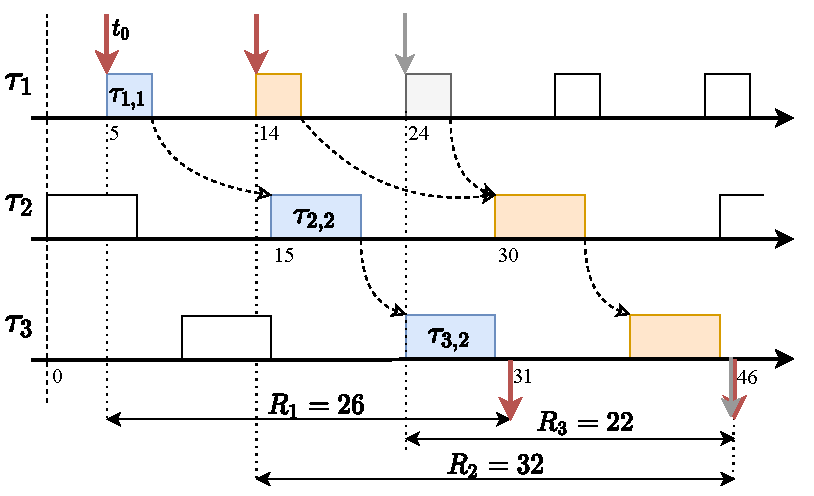
\includegraphics[width=.8\linewidth]{TaskChain_chronogram.pdf}
	    	\caption{Exemple d'exécution d'une chaîne de tâches $\tau_1 \rightarrow \tau_2 \rightarrow \tau_3$}
	    	\label{fig:chain_chronogram}
	    \end{figure}
    
	    Dans ce contexte, on peut donc définir la relation entre une tâche $\tau_i$ et son successeur $\tau_{i+1}$. Pour produire la donnée de sortie du job $\tau_{i+1,k}$ de la tâche $\tau_{i+1}$, ce dernier consommes toutes les données d'entrée en attente provenant des jobs $\tau_{i,j}$. Les données en attente étant celles qui n'ont pas été consommé par le job précédent de $\tau_{i+1}$, i.e. $\tau_{i+1,k-1}$. On peut donc écrire que pour un $\{i,k\}$ donnés, sont consommés les données de tous les jobs $\tau_{i,j}$ ssi $j \textup{ tel que } e_{i,j} \leq s_{i+1, k}$ et $e_{i,j} > s_{i+1, k-1}$. Autrement dit, un job $\tau_{i,j}$ n'a un effet sur $\tau_{i+1,k}$ si et seulement si ce dernier est le premier job de $\tau_{i+1}$ exécuté après la terminaison de $\tau_{i,j}$.
	    
		Dans ces conditions, on nomme $\tau_{i+1,k}$ le \textbf{successeur} du job $\tau_{i,j}$. On note $succ()$ la fonction qui permet de trouver le successeur d'un job donné. Par extension, la fonction itérative $succ^{n-1}()$ permet de trouver le job de sortie d'une chaîne de tâche donnée, selon le job d'entrée. 
	    Pour illustrer cela, on peut prendre l'exemple d'une chaîne de trois tâches $\tau_1 \rightarrow \tau_2 \rightarrow \tau_3$, tel que représenté en~\autoref{fig:chain_chronogram}. On peut par exemple voir qu'une des exécutions de la chaîne de tâche, débutant par $\tau_{1,1}$, donne : $succ^{2}(\tau_{1,1}) = succ(succ(\tau_{1,1})) = succ(\tau_{2,2}) = \tau_{3,2}$. Mais aussi que le job $ \tau_{2,3} $ doit prendre en compte les valeurs de sorties de 2 jobs de la tâche $ \tau_1 $. %On a alors le temps de réponse de la-dite chaîne : $R_1 = e_{3,2} - s_{1,1} = 31 - 5 = 26$ unités de temps.
	    
  		Étant donné que les tâches peuvent être définies par des périodes d'activation différentes, cela signifie notamment que si une tâche $\tau_i$ est exécutée plus fréquemment que son successeur $succ(\tau_{i+1})$, alors il est possible  qu'un job $\tau_{i+1,j}$ soit le successeur de plusieurs jobs de la tâche $\tau_{i}$. Cette façon de considérer les choses permet une plus grande flexibilité de notre modèle pour s'adapter à un cas concret. En effet, de cette façon le modèle gère déjà un nombre assez significatif d'implémentations de tâches existantes~:
	\begin{itemize}
		\item   		les tâches qui ne considèrent que la donnée d'entrée la plus récente, les données précédentes étant considérées obsolètes. Dans ce cas-là, si les données de 2 jobs prédécesseurs sont consommés, en réalité la donnée du job le plus ancien des deux sera simplement ignorée.
		\item   		Les tâches avec une file d'attente en entrée : lorsque la tâche est exécutée elle consomme toutes les données d'entrée en attente.
		\item   		Pour les tâches où chaque exécution de la tâche ne prend en compte qu'une seule donnée de la file d'attente, ce n'est géré que partiellement. Cela peut être la donnée la plus ancienne (stratégie FIFO\footnote{FIFO : First-In First-Out, les données sont traitées de la première arrivée à la dernière.}) ou la plus récente (stratégie LIFO\footnote{LIFO : Last-In First-Out, les données sont traitées de la dernière (plus récente) arrivée à la plus ancienne.}). Si une tâche s'exécute plus lentement que sa prédécesseure, c'est le cas que nous ne gérons pas. Cependant, il est improbable, car cela implique que la quantité de données en file d'attente peut potentiellement exploser (or, la file d'attente ne peut être infinie). En revanche si les tâches ont toutes la même fréquence d'activation, ou si les tâches prédécesseures s'exécutent systématiquement à une plus faible fréquence que les tâches suivantes, alors on se retrouve finalement dans la même situation que le premier type de tâches citées. De fait cela implique qu'il n'y a en réalité jamais plusieurs données en attente à l'entrée en fonctionnement normal. 
	\end{itemize}
  		De façon succincte, quand on parle de "consommer" plusieurs jobs de la tâche précédente tel qu'on le présente ici, cela n'implique pas que toutes ces données seront prises en compte. Tout dépend du modèle de fonctionnement interne des tâches. Mais quoi qu'il en soit, cela permet de gérer un grand nombre de comportements classiques.
  		
  		Ce modèle présente en revanche un inconvénient qui est de ne pas considérer de potentiels retards entre le moment où une tâche délivre sa donnée de sortie et le moment où cette donnée est réellement disponible pour son successeur. Il faudrait pour cela ajouter une constante de latence correctement estimée selon le système à la condition de précédence de tâche.
	    %%i.e. un \textit{job} $k$ donné de la tâche $i+1$ consomme toutes les données des \textit{jobs} de la tâche $i$ qui se sont terminées avant le début de son exécution et qui n'ont pas été consommées par le job précédent $k-1$.


        \paragraph{Temps de réponse bout-en-bout}

    La notion de successeur permet de définir le temps de réponse bout-en-bout $R_j$ de la $ j^{eme} $ instance d'exécution d'une chaîne de tâche. Ainsi $ R_j $ désigne le temps écoulé entre l'activation du \textit{job} d'entrée $\tau_{1, j}$ de la chaîne, jusqu'à la terminaison du \textit{job} de sortie $\tau_{n, k} = succ^{n-1}(\tau_{1, j})$.
    On a alors $R_{j} = e_{n,k} - a_{1,j}$ que l'on peut retrouver dans l'exemple du~\autoref{fig:chain_chronogram}. Sur cet exemple, il est possible de reconstituer trois instances d'exécution de la chaîne de tâche avec les trois temps de réponse correspondants : $R_1$, $R_2$, $R_3$. 
    %Parmi ces instances, on remarque que 2 d'entre-elles sont très semblables, avec le même job de terminaison $ \tau{3,3} $.
    
	Intuitivement, l'échéance bout-en-bout représente alors la durée maximale acceptable pour qu'une donnée d'entrée de la chaîne ait un effet du côté de la sortie. Pour une fonctionnalité donnée on comprend bien que cette échéance doit être bornée, et qu'il faut donc des garanties pour que tout se passe bien bout-en-bout. À considérer l'échéance d'une chaîne de tâche $D$, pour éviter toute faute temporelle de non-respect d'échéance, il faut a minima respecter~:  $\max_{j \in \mathbb{N}}\{R_j\} \leq D$.
	
	\smallbreak 
	
	L'objectif à présent est de proposer une approche qui permette justement d'exploiter ces contraintes bout-en-bout, de façon à éviter les risques de fautes temporelles au niveau fonctionnel. Cela se traduit par la volonté de prévenir les risques de dépassement d'échéances, non pas au niveau de chaque tâche individuelle mais plutôt à un niveau d'observation au-dessus qui est en lien direct avec la représentation fonctionnelle.
	
    
\section{Mécanisme d'anticipation par Surveillance et Contrôle}
    \subsection{Méthode d'anticipation}
    
    Je propose donc un mécanisme basé sur la surveillance à l'exécution de l'avancement d'une chaîne de tâche. 
    Pour ce faire, on introduit les notions d'\textbf{État de Chaîne de Tâche} et de \textbf{Trace d'Exécution de Chaîne de Tâche}. Une chaîne de tâche donnée est associée à un État et plusieurs Traces d'Exécutions. Ces deux éléments évoluant au fil de l'exécution du système, on peut noter $S_C(t)$ l'État et $ET_C(i,t)$ une Trace d'Exécution donnée de la Chaîne de tâches.
    
    On peut alors définir pour une Chaîne de Tâche dont la tâche d'entrée est $\tau_{1}$, et la tâche de sortie $\tau_{n}$ : 
    \begin{definition}
    	Une \textbf{Trace d'Exécution} $ET_C(i)$ se définit par un job d'entrée ainsi que tous les \textit{successeurs} itératifs de ce job. \\
    	\begin{equation*}
    		S_C(i) = \{ \tau_{1,i} \:,\: succ(\tau_{1,i})\:, \;\dots\; ,\: succ^n(\tau_{1,i}) = \tau_{n,i} \}
    	\end{equation*} \\    	
    	À un instant $t$, une Trace d'Exécution est dite \emph{active} si son job de départ $\tau_{1,i}$ a déjà été activé, et que son successeur itératif correspondant à la tâche de sortie de la chaîne $\tau_{n,i}$ n'a pas encore été terminé. Autrement, elle est \textit{inactive}. En d'autres termes : \\
    	\begin{equation*}
    		TE_C(i,t)  \quad \textrm{est active ssi}\quad  a_{1,i} \leq t \quad \textrm{et} \quad e_{n,i} > t
    	\end{equation*} 
    \end{definition}
    
    %Our anticipation mechanism is based on the run-time monitoring of the task chain progress. 
    %To that end, we introduce the notions of \textbf{Task Chain State} and \textbf{Task Chain Execution Trace} (TCET). 
    %A TCET contains an entry task job and all the iterative successors of that job. 
    %At a time $t$ a TCET can be \emph{active}, if its entry task job has been activated and if its exit task job has not yet ended, or \emph{inactive} otherwise. 
    
    À un moment $t$ de l'exécution du système, il est possible de définir à partir de l'état des Traces d'exécution (actives ou inactives) l'État de la Chaîne de tâches : 
    \begin{definition}[Etat d'une Chaîne de Tâche]
    	L'État d'une Chaîne de Tâche définie à un instant $t$ l'état d'avancement de l'exécution de la chaîne de tâche qui est toujours en cours et a été activée la plus anciennement. En d'autres termes : 
    	\begin{equation*}
    		S(t)=\langle t_0, \tau_i\rangle
    	\end{equation*}
    Avec $t_0$ la plus ancienne activation parmi les $ET_C(i,t)$ et $\tau_i$ la prochaine tâche de cette trace d'exécution qui n'a pas encore été exécutée.
    \end{definition}
    De cette façon, l'État d'une chaîne de tâches indique quelles sont les tâches restantes à exécuter dans la chaîne à un instant donné et son temps de réponse partiel actuel que l'on notera $RT(t) = t - t_0$.
    
    Pour finir, au regard de l'État d'une chaîne de tâches, on peut s'intéresser au temps restant à la complétion de cette chaîne. Il est possible d'estimer le temps qu'il faudra pour aller jusqu'à exécuter la tâche de sortie de la Trace d'Exécution active observée. Et si de plus cette estimation est faite dans la même logique qu'une estimation de Temps d'Exécution Pire Cas, on obtient alors une estimation de \textbf{\emph}{Pire Temps de Réponse restant} $rWCRT(t)$ à l'instant $t$.
    
    Alors, en combinant l'État à un instant $t$ avec une estimation du Temps de Réponse Pire Cas restant, on peut donc estimer une borne haute garantie de temps de réponse de la chaîne de tâche. C'est là que l'on peut faire entrer en jeu un mécanisme d'anticipation. 
    On dispose pour une chaîne de tâches donnée de son temps de réponse partiel actuel ainsi qu'une estimation de temps de réponse restant en pire cas. Il est alors possible de déterminer s'il y a un risque de défaillance par dépassement de l'échéance bout-en-bout $D$.
    \begin{theorem}[Risque de dépassement d'échéance]
    	Si à un instant donné $t$, l'inéquation suivante est respectée, alors il y a risque de dépassement d'échéance.
    	\begin{equation*} 
    		RT(t) + rWCRT(t) \geq D_C
    	\end{equation*}
    \end{theorem}

	Pour illustrer cette logique, on peut voir sur le chronogramme~\ref{fig:chronogram_rWCRT_example} à nouveau un exemple avec une chaîne de tâche $\tau_1 \rightarrow \tau_2 \rightarrow \tau_3$. À l'instant $t=18$ indiqué il y a deux Traces d'Exécution actives (chaînes reliées par une flèche de succession). On a de ce constat l'État de la chaîne $S_C(t) = \langle \tau_0, \tau_2\rangle = \langle 5, \tau_{2} \rangle $.
	On en déduit $ RT(18) = t - t_0 = 18-4 = 14 $. Si l'on ajoute à cela une estimation du Temps de Réponse Pire Cas restant $rWCRT(\tau_i)$, qui est le temps estimé pour que $\rightarrow \tau_2 \rightarrow \tau_3$ soit exécuté selon les contraintes de précédence, alors on a l'estimation du Pire Temps de Réponse : $ RT(18) + rWCRT(18) = 33$ que l'on peut comparer à la date d'échéance $ D_c = 30 $. Dans cet exemple, il existe donc un risque de dépassement de l'échéance.
	Il est à noter aussi que dans cet exemple l'instant $t$ a été pris en plein pendant l'exécution de la tâche $ \tau_2 $. Ce qui est pris en considération comme si cette dernière n'était pas exécutée. Si l'on ne prend pas non plus en compte son exécution partielle, c'est parce que d'un point de vue externe à cette tâche, sans l'instrumentaliser il n'est pas possible de le savoir. Et de fait, l'une de nos contraintes étant d'être le moins intrusif possible sur le code, notamment pour les cas où certains logiciels ne sont pas modifiables (black-box ou legacy). 
	
    \begin{figure}[ht]
		\centering 
		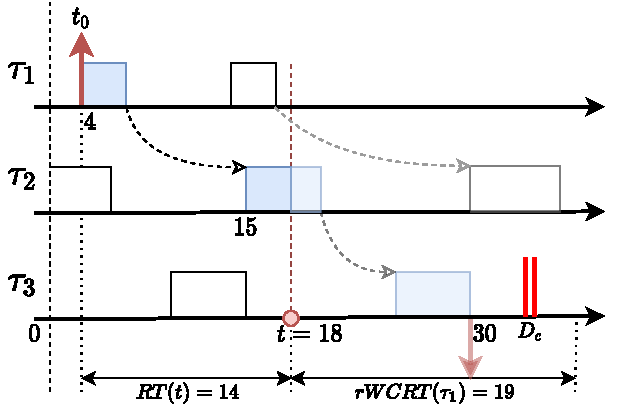
\includegraphics[width=0.7\linewidth]{chronogram_rWCRT_example.pdf}
		\caption{Exemple de trace d'exécution et Etat de la Chaîne pour anticipation}
		\label{fig:chronogram_rWCRT_example}
	\end{figure}

	À présent, il faut nous souvenir de notre objectif dans tout cela. Pourquoi vouloir anticiper une défaillance de la sorte ? Pour rappel l'objectif est d'anticiper un risque de dépassement d'échéance à l'échelle d'une chaîne de tâches, de façon à pouvoir passer d'un Mode d'ordonnancement Nominal vers un mode Dégradé dans lequel on va prévenir la défaillance. Cette dernière a pour origine première les interférences matérielles qui augmentent les temps d'exécution des tâches. Aussi pour éviter davantage ce rallongement et donc conserver la garantie de terminaison de la chaîne de tâche avant l'échéance, on remonte à la source en prévenant temporairement tout risque d'interférences. Et cela est obtenu via un mode dégradé dans lequel la méthode consiste à stopper temporairement les tâches non critiques, cause des interférences.
	Il nous faut donc prendre en compte la méthode de passage en mode dégradé. 
	

    
    \subsection{Passage en Mode Dégradé}
    
        \paragraph{Estimation de Temps d'Exécution Pire Cas restant}
    Bien évidemment, l'estimation du Temps de Réponse Pire Cas restant est un élément clé de l'approche. Tout l'intérêt de cette méthode réside dans la capacité à passer dans un mode dégradé. En conséquence, ce que nous nous devons de garantir, c'est le non-dépassement d'échéance sachant qu'il est possible à tout moment de prendre la décision du passage en mode dégradé, dans lequel les tâches critiques n'étant plus sujettes à interférences externes, auront un Temps d'Exécution Pire Cas bien plus faible qu'en mode Nominal. 
    Cela implique directement que si le $rWCRT(\tau_i)$ que nous considérons est dans le contexte Dégradé, alors la détection d'un éventuel risque se fait de façon beaucoup plus permissive que si l'on considère directement les risques en mode Nominal.
    
    Il existe plusieurs méthodes à son obtention. 
    De façon théorique, il est possible d'exploiter les méthodes déjà existantes d'estimation de temps d'exécution pire cas, auxquelles il faut ajouter la prise en compte des temps d'activation des tâches. Ce type d'approche devient hautement dépendante du système étudié, que ce soit l'architecture matérielle, mais surtout la politique d'ordonnancement des tâches, le type de tâches (périodique, sporadique, interruption)... De façon générale, la complexité des approches théoriques n'est pas négligeable et, il faut l'admettre, hors de notre cadre d'expertise. C'est d'autant plus vrai dans un cas d'application sur processeur multicœur pour lequel il est facile de tomber dans des estimations trop pessimistes. Pour cette raison, nous avons décidé dans notre proposition d'avoir une approche plus expérimentale.
    
    %To help with the estimation of $rWCRT$, we assume that the HI-criticality task chain execute on a single core. To avoid interference between the MCA and the task chain we prevent the MCA to use the same core. Lo-criticality tasks can execute on any core as depicted on \autoref{fig:SoftwareArchitecture}. 
    
    Un avantage dont nous bénéficions ici, c'est que l'hypothèse de se ramener à un cas en isolation dans le mode dégradé limite grandement les risques de variations sur les temps d'exécutions des tâches critiques. C'est ce qui permet une plus grande certitude sur les estimations expérimentales, qui ne nécessitent alors plus de couvrir toute une combinatoire incluant les tâches non critiques. L'estimation est donc faite expérimentalement en exécutant le système avec un passage forcé en mode dégradé dans lequel on peut alors mesurer sans les tâches non-critiques les Temps de Réponse Pire Cas restants $rWCRT(\tau_i)$. On notera que pour une chaîne de N tâches, il y a N-1 rWCRT à estimer. Plus de détails sur le protocole adopté pour l'estimation seront abordés en~\autoref{chap:4_ProtocolExpe}. 
    
    Il reste à aborder à présent la transition en elle-même vers le mode dégradé. Cette phase est importante du fait qu'elle implique des délais supplémentaires qui devront être pris en compte dans l'anticipation. De cette façon, à considérer que l'on recalcule périodiquement le risque de dépassement d'échéance, il est possible de définir l'instant où l'on sait que l'attente d'une période supplémentaire va faire que même en mode dégradé, il ne sera plus possible de garantir le respect de l'échéance bout-en-bout. Par conséquent, il devient alors clair que cet instant-là devient le dernier moment auquel il faut nécessairement passer en mode dégradé pour justement conserver cette garantie.
        
	\paragraph{Transition de Mode}
    Ce changement de mode se fait en 3 étapes. Il faut en premier lieu bien entendu la détection du point de bascule auquel le risque de défaillance est détecté, c'est l'étape de décision. Une fois la décision prise, la seconde étape est d'activer le mécanisme de passage en mode dégradé. Dans notre cas, il s'agit d'envoyer un signal aux tâches non critiques de façon à mettre en pause leur exécution, c'est l'étape de contrôle. Enfin, le système de surveillance doit continuer d'observer l'État de la chaîne de tâche de façon à relancer les tâches non critiques une fois le risque passé. Il s'agit de l'étape de recouvrement.
    
    Ces trois étapes font ressortir un élément important pour l'anticipation qui n'a pas été pris en compte pour le moment, et il s'agit de la durée entre l'étape de décision et la fin de l'étape d'exécution. En effet, le temps pour que toutes les tâches non critiques soient mises en pause est non nul, et ce délai doit être pris en compte dans l'estimation de Temps d'Exécution Pire Cas restant dans l'optique où le pire cas en question est considéré dans le mode dégradé.
    
	En conclusion, en considérant les grandeurs suivantes : 
	\begin{itemize}
		\item 	$ W_max $ La durée maximum garantie entre 2 points de surveillance de l'Etat de la chaîne de tâche
		\item 	$ t_{SW} $ Le délai maximum nécessaire à la transition du mode nominal au mode dégradé
		\item 	$ rWCRT(\tau_i) $ pour chaque $\tau_i$ de la chaîne de tâche, les Temps de Réponses Pire Cas restant en mode dégradé
	\end{itemize}
	Il est alors possible de calculer la somme du temps de réponse partiel actuel avec ces trois métriques. Tant que cette somme reste inférieure à l'échéance bout-en-bout, alors on peut conserver le système en mode nominal. En revanche, à partir du moment où cela dépasse l'échéance, alors c'est le moment où il n'est plus sûr de rester en mode nominal, et il faut donc déclencher le mode dégradé pour garantir le respect de l'échéance. Cela correspond en conséquence à surveiller que l'inéquation suivante reste vraie pour savoir l'instant critique auquel il faut passer en mode dégradé~:
	\begin{equation} \label{safe_cond}
		RT(t) + rWCRT(\tau_i) + W_{max} + t_{SW} \leq D
	\end{equation} 
	Cette équation est notamment adaptée des travaux de~\cite{kritikakou_run-time_2014}. Chaque point de surveillance de l'État de la chaîne de tâches est considéré comme étant temporellement sûr (au sens où il n'y a pas de risque de faute temporelle due au dépassement d'échéance) tant que cette inégalité est respectée.
    
    \begin{proof}
		En présumant que (\ref{safe_cond}) est respectée, on peut montrer qu'il est sûr d'attendre le prochain point de surveillance pour décider de changer de mode. Soit $t_{next}$ le prochain instant de surveillance.
		Par définition, $t_{next} \leq t + W_{max}$ alors nécessairement $RT(t_{next}) \leq RT(t) + W_{max}$, par conséquent  \\
		$RT(t_{next}) + rWCRT(\tau_i) + t_{SW} \leq RT(t) + rWCRT(\tau_i) + W_{max} + t_{SW}$. \\
		Aussi, $rWCRT()$ ne peut que décroître avec le temps qui s'écoule, par conséquent
		\[ rWCRT(t_{next}) \leq rWCRT(\tau_i)	\]
		et 
\[ RT(t_{next}) + rWCRT(t_{next}) + t_{SW} \leq RT(t) + rWCRT(\tau_i) + W_{max} + t_{SW} \] 
		Étant donné que (\ref{safe_cond}) est respecté, on a $RT(t_{next}) + rWCRT(t_{next}) + t_{SW} \leq D$.
		De ce fait, il sera sûr de passer en mode dégradé au prochain point de surveillance.  
    \end{proof}
    
    \begin{figure}[ht]
    	\centering
    	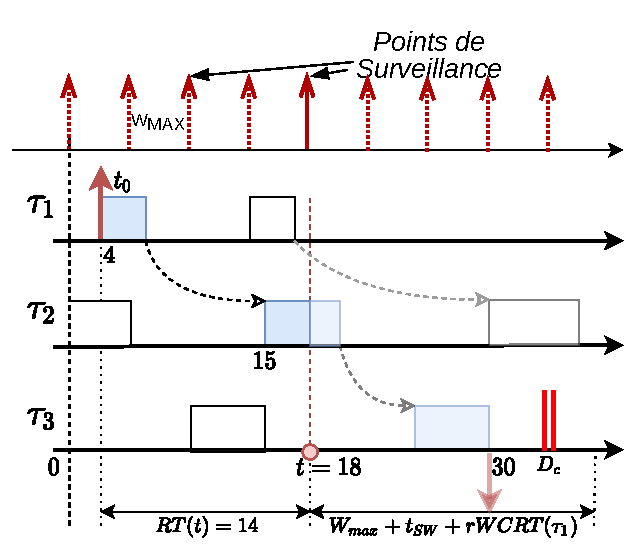
\includegraphics[width=0.7\linewidth]{schemas/chronogram_rWCRT_complet}
    	\caption{}
    	\label{fig:rwcrtchronogram}
    \end{figure}

    En adaptant ce qui a été présenté précédemment avec le risque de dépassement d'échéance, on peut retrouver en~\autoref{fig:rwcrtchronogram} l'ajout des composants qui permettent l'anticipation du changement de mode, au regard de la période de surveillance et du temps de changement.
	La méthode de réglage de la période de surveillance sera discuté dans le~\autoref{chap:4_ProtocolExpe}.
	
	\section{Architecture Logicielle}
	
	Maintenant que nous avons présenté toute la logique derrière le mécanisme de surveillance et de contrôle, nous allons présenter plus en détail l'architecture logicielle nécessaire à son implémentation.
	
	Pour résumer la situation, nous sommes dans le cas d'un système implémenté sur un calculateur multicœur, dans lequel nous avons distingué une chaîne de tâche critique des autres tâches considérées non-critiques. Il faut bien entendu ajouter à cela un Agent de Surveillance et de Contrôle pour assurer la fonctionnalité de mitigation des fautes temporelles. Ce dernier se destine à être exécuté en couche bas niveau, au même niveau que la politique d'ordonnancement du système. Dans le cadre de la suite de nos expérimentations, pour simplifier l'implémentation, nous avons considéré l'isolation de l'Agent de Surveillance et Contrôle sur un cœur du processeur. L'ensemble de ces éléments se résume en~\autoref{fig:SoftwareArchitecture}.

\begin{figure}[ht]
            \centering
            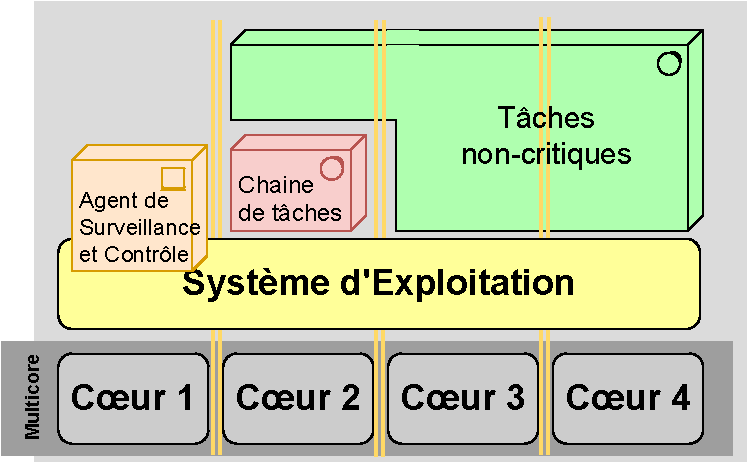
\includegraphics[width=.7\linewidth]{ArchitectureLogicielle.pdf}
            \caption{Monitoring \& Control Agent basic concept} \label{fig:SoftwareArchitecture}
\end{figure}

	L'Agent de Surveillance et Contrôle peut se décomposer en deux éléments distincs. D'un part un \emph{Task Wrapper Component} (TWC) et de l'autre le \emph{Core Control Component} (CCC). Le TWC se destine à récupérer toutes les informations nécessaires à la surveillance et la mise à jour de l'État de la Chaîne de tâche, tandis que le CCC doit prendre en compte ces informations, de façon à réaliser la prise de décision du passage en mode dégradé au regard de l'inéquation~\ref{safe_cond}.
	
	
        \begin{figure}[ht]
            \centering
            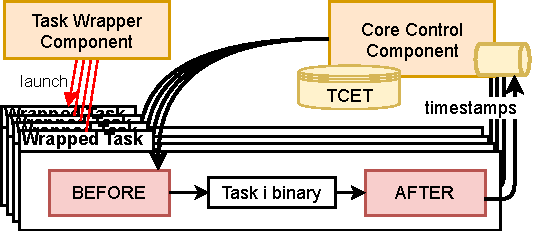
\includegraphics[width=0.7\linewidth]{ArchitectureFramework.pdf}
            \caption{Monitoring \& Control Agent Architecture\label{fig:architecture}}
        \end{figure}
        
        
        \subsection{Task Wrapper Component (TWC)} 
        
        It is responsible for encapsulating the system tasks between two software wrappers, ``Before" and ``After". Those wrappers have two roles: \begin{itemize}
                \item provide timestamps (start and end of HI tasks) to the Core Control Component.
                \item prevent LO tasks execution in HI-criticality mode.
            \end{itemize}
            
%%%%%%%%%%%%%%%%%%%%%%%%%%%%%%%%%%%%

        The timestamps are queued to be processed by the Core Control Component to update the TCET.
        The ``Before" wrapper is also used to prevent LO task execution in degraded mode. There is no need for an ``After" wrapper for LO tasks.

        \subsection{Core Control Component (CCC)}
           The Core Control Component executes with a period $T_{ccc}$. It updates each \textbf{active Task Chain Execution Trace} (TCET), taking into account timestamps received since its last execution and compute the task chain state $S(t)$, enabling the evaluation of $RT(t)$ and $rWCRT(\tau_i)$. Then CCC checks if inequality~(\ref{safe_cond}) is still true. If not, the CCC switches to degraded mode to guarantee the task chain deadline. The mode switch is realised through two actions: sending a Pause signal to every LO-criticality tasks, and signaling ``Before" wrapper to prevent any new execution.
        
\cmnt{
            The Core Control Component stores each active \textbf{Task Chain Execution Trace} (TCET) in order to compute the task chain state $S(t)$ at any time.
            
            %The Core Control Component updates the task chain timing state periodically to check if the deadline can still be guaranteed. The $S(t)$ update frequency is fixed and not directly triggered by a monitoring message (i.e. at one update we could have multiple pending finished tasks to consider or none). Consequently, such period must be chosen regarding the tasks' execution times to avoid having too much monitoring messages to take into account. 
            Task chain state updates are triggered periodically, every $T_{ccc}$, and not asynchronously (for each new monitoring message) to avoid being dependent on when the ``Before" and ``After" wrapper are executed. This way we can still decide to switch to degraded mode as ET(t) still increases as we are getting closer to the deadline even with no new monitoring message.
            
            At each TCET update, the CCC check if inequality~\ref{safe_cond} is still true. If not, the CCC switches to degraded mode to guarantee the task chain deadline. The mode switch is made first by sending a Pause signal to every non-critical task from the CCC, in addition to the TWC blocking feature mentioned above.
        }
        
            The CCC parameters $t_{sw}$ and $W_{max}$ are important to define. If those parameters are underestimated, then it is not safe to use inequality~(\ref{safe_cond}). We estimate them for our experimental platform in \ref{expe_calibPhase}. 
            $W_{max}$ is the maximum duration between two CCC checkpoints. It is directly dependent to the CCC period $T_{ccc}$. If Hi-criticality tasks are periodic, which is typical, it is simple to set this value, around the smallest task period. This way we have the guarantee of not overflowing the timestamps queue used by the CCC. A greater value is possible, but we must take care to process the $TCET$ updates faster than the arrival of timestamps. For other tasks activation models, we must identify the highest task timestamps arrival rate to avoid any queue overflow. 
            It is also important to set $T_{ccc}$ --and thus, $W_{max}$-- as it will directly influence the sensitivity of our anticipation mechanism. With a higher CCC update frequency --and consequently a lower $W_{max}$-- we switch to degraded mode later. Also, it will naturally use more computing resources. A higher value triggers sooner and may increase the number of unneeded switches to degraded mode (i.e. false positives). 
            %Future work could aim at measuring more precisely $W_{max}$ influence. 

        \cmnt{
            One should note that what makes such approach possible is the evolution of the $rWCRT$ at run-time and as the $S(t)$ evolves. It would not be possible to apply such approach when it comes to monitor \& control individual tasks to guarantee their individual deadlines. For individual deadlines, our method would fit only if we are able to monitor tasks timing state ``inside" the tasks execution, i.e. instrumenting the tasks source code to add internal checkpoints. Such approach on individual tasks would discard by definition the use of black box software assumption for instance, and otherwise would need much higher refresh rate frequencies in order to follow individual tasks execution timing state. Such solution is presented for individual tasks in~\cite{kritikakou_dynascore_2017}.
            }
            
\section{Application au domaine  automobile (diag. fonctionnel, SWC, etc)}
    \subsection{Concept Description}
        Our approach presents a software execution \emph{Monitoring and Control Agent (MCA)} to guarantee end-to-end deadline constraints.
        %Our challenge is to investigate that an appropriate combination of general-purpose scheduling policies, tasks allocation to cores, freezing strategies of non-critical tasks when critical tasks need more computing resources is a solution to comply with end-to-end real-time constraints. %In practice deadline specifications are often arbitrary and approximate due to system complexity. 
        We focus on the respect of end-to-end constraints of tasks chains, not individual tasks constraints. The idea behind this is to offer more ``flexibility'' on tasks scheduling for guaranteeing mandatory task chains constraints if we control only end-to-end constraints instead of every critical task timing constraint. By doing so, we gain "flexibility" as we allow some parts of the chain to be behind time as they can be compensated before the end of the chain without any external action. The MCA monitors at run-time the execution time of critical tasks and anticipate when the end-to-end deadlines may be compromised to stop non-critical tasks when needed in order to avoid such risk. The anticipation is based on the estimation of remaining WCET. Finally, when the critical task chain recovers from the potential risk, the non-critical tasks can resume their execution to get back to a nominal state.
        
        We define a \textit{degraded mode}, opposed to the \textit{nominal mode} of execution. In nominal mode, critical and non-critical tasks are executed normally. In Degraded mode, non-critical tasks are not executed, to prevent further interferences on critical tasks. The degraded mode implies simpler WCET estimations because we eliminate the disturbances from non-critical tasks; such WCET will be lower than in a nominal mode. It is probably less pessimistic as we eliminate memory interferences, non-critical tasks scheduling and possible common resources (drivers for instance) usage. The main disturbances remaining will be only between the tasks from the chain. Consequently, our anticipation mechanism will be based on reduced estimation of WCET (compared to nominal mode), to activate degraded mode only as a last resort.
        \smallbreak
        To reach degraded mode, MCA role is to pause/stop non-critical tasks execution. This control is triggered by an anticipation algorithm. To be efficient, this algorithm should trigger the control at the latest possible time while guaranteeing real-time end-to-end constraints.
        
        %Individual deadline could be compromised however the goal is to respect task chains deadlines.
        %Individual WCET are also useful, but if they are not available, approximations extracted from behavioral models are enough, for example with an equal distribution of the global end-to-end time value as described in [ref].  
        \begin{figure}[h]
            \centering
            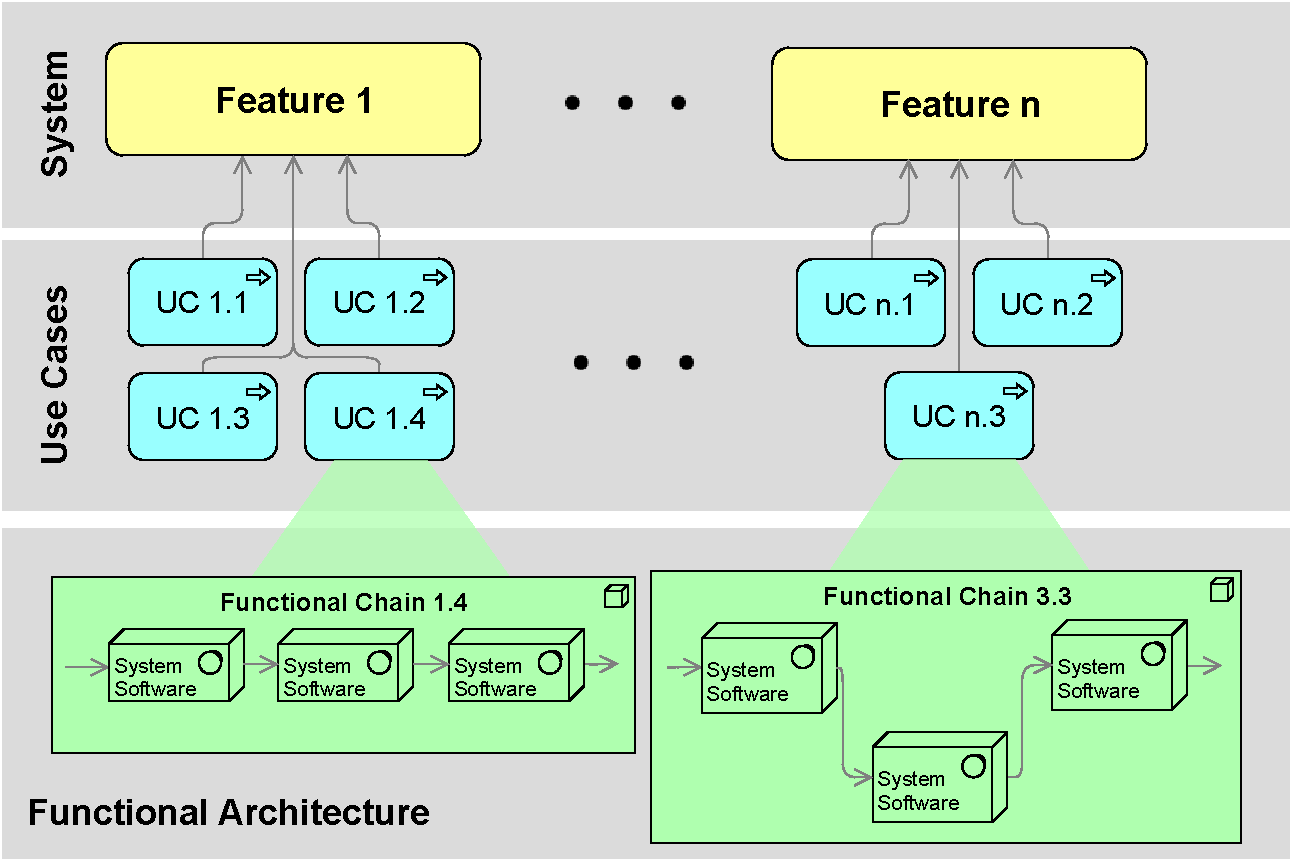
\includegraphics[width=\linewidth]{SchemaChaineFonctionnelle}
            \caption{Functional Architecture definition} \label{fig:funcArch}
        \end{figure}
        \smallbreak
        \subsubsection{Functional Specification} 
            A critical task chain must describe the implementation of a system functionality from its triggering to its consequence. This would stick most of the time with a computing chain going from a sensor measure to an actuator command. First idea would be to stick with safety criticality levels (ASIL D to ASIL A and QM, for automotive applications), but we quickly notice that there is no direct link between this classification and critical tasks chains. A safety critical task is not necessarily defined from its timing constraints. The only possible conclusion here is that a critical task chain only includes non-QM tasks. 
            \smallbreak
            We propose here a definition based around high-level specifications as represented in figure~\ref{fig:funcArch}. The global system is defined as a set of features\footnote{Features: all the services the system must provide. e.g: Lane Support System (LSS) is a feature.}. Every feature gathers a set of functionalities that are translated into Use Cases\footnote{e.g: Lane Departure Warning \& Lane Keeping Assist are part of the use cases of LSS feature.}. A Use Case defines a feature behavior for a given context and inputs (and the consequent outputs). Finally, those are translated into functional chains representing different functions and their interactions needed for the realization of the Use Case. 
            
            If we combine this information with a severity classification in case of failure of the use cases, it is possible to define critical chains as functional chains with a high severity risk. This is one possible criterion allowing an easy separation between a critical functional chain and the others. It could be adapted during the design phase, depending on the functional chains allocated to the processor. 
            \smallbreak
            Such information allows to define the software components involved in the critical task chain. All the software components used to realize a critical functional chain form a critical task chain at an OS point of view. At this point, it is possible to define the task chain end-to-end deadline, following the severity temporal risk in case of failure. Such deadline should be at minimum the sum of individual tasks deadline, but could probably be higher, depending on the global system and the task chain function. Our objective is to guarantee such critical task chain end-to-end execution time on the multicore.
\ifdefined\included
\else
\bibliographystyle{StyleThese}
\bibliography{these}
\end{document}
\fi
